\documentclass[11pt,compress,t,notes=noshow, aspectratio=169, xcolor=table]{beamer}

\usepackage{../../style/lmu-lecture}
% Defines macros and environments
% This file is included in slides and exercises

% Rarely used fontstyle for R packages, used only in 
% - forests/slides-forests-benchmark.tex
% - exercises/single-exercises/methods_l_1.Rnw
% - slides/cart/attic/slides_extra_trees.Rnw
\newcommand{\pkg}[1]{{\fontseries{b}\selectfont #1}}

% Spacing helpers, used often (mostly in exercises for \dlz)
\newcommand{\lz}{\vspace{0.5cm}} % vertical space (used often in slides)
\newcommand{\dlz}{\vspace{1cm}}  % double vertical space (used often in exercises, never in slides)
\newcommand{\oneliner}[1] % Oneliner for important statements, used e.g. in iml, algods
{\begin{block}{}\begin{center}\begin{Large}#1\end{Large}\end{center}\end{block}}

% Don't know if this is used or needed, remove?
% textcolor that works in mathmode
% https://tex.stackexchange.com/a/261480
% Used e.g. in forests/slides-forests-bagging.tex
% [...] \textcolor{blue}{\tfrac{1}{M}\sum^M_{m} [...]
% \makeatletter
% \renewcommand*{\@textcolor}[3]{%
%   \protect\leavevmode
%   \begingroup
%     \color#1{#2}#3%
%   \endgroup
% }
% \makeatother


\title{Interpretable Machine Learning}
% \author{LMU}
%\institute{\href{https://compstat-lmu.github.io/lecture_iml/}{compstat-lmu.github.io/lecture\_iml}}
\date{}

\begin{document}

\newcommand{\titlefigure}{figure/ale_plot.pdf}
\newcommand{\learninggoals}{
\item PD plots and its extrapolation issue
\item M plots and its omitted-variable bias
\item Understand ALE plots
}

\lecturechapter{Accumulated Local Effect (ALE): Introduction }
\lecture{Interpretable Machine Learning}
%
% \frame{
% \frametitle{Motivation}
%
% \begin{columns}[T, totalwidth=\textwidth]
% \begin{column}{0.5\textwidth}
% \centering
% \includegraphics[width=\textwidth]{figure_man/ale_scatter}
% \end{column}
% \begin{column}{0.5\textwidth}
% \centering
% \includegraphics[width=\textwidth]{figure_man/ale_pdplot}
% \end{column}
% \end{columns}
%
% \only<1>{
% \textbf{Recall:} In case of strongly correlated features $x_1$ and $x_2$, partial dependence (PD) plots \textbf{average predictions} of artificial data instances that are unlikely in reality (green).
% This can lead to biased estimates.
%
% \textbf{Question:} Can we avoid the extrapolation issue by averaging only over points in an appropriate neighborhood? % of a specific point $x_1$? %, i.e., using the conditional distribution at
% }
%
% \only<2>{
%
% \textbf{Answer:} Yes, we could. Marginal plots (M plots) do this by averaging (i.e., marginalizing) over the conditional distribution $\P(\xv_2|x_1)$.
%
% \textbf{But:} M plots introduce the omitted-variable bias (OVB) issue, i.e., an
% M plot always includes the marginal effect of other dependent features.\\
% $\Rightarrow$ M plots are useless to assess the main effect of a feature.
%
% }
% }



\begin{frame}{Motivation - Correlated Features}

\begin{columns}[T, totalwidth=\textwidth]
\begin{column}{0.5\textwidth}
\centering
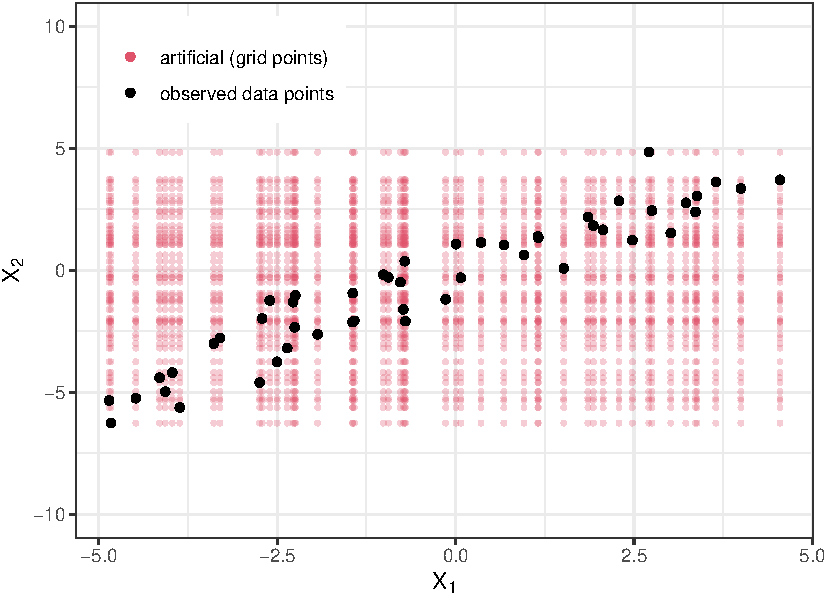
\includegraphics[width=0.9\textwidth]{figure/ale_scatter_grid}
\end{column}
\begin{column}{0.5\textwidth}
\centering
\includegraphics[width=0.9\textwidth]{figure/ale_pdplot}
\end{column}
\end{columns}

%\begin{center}
%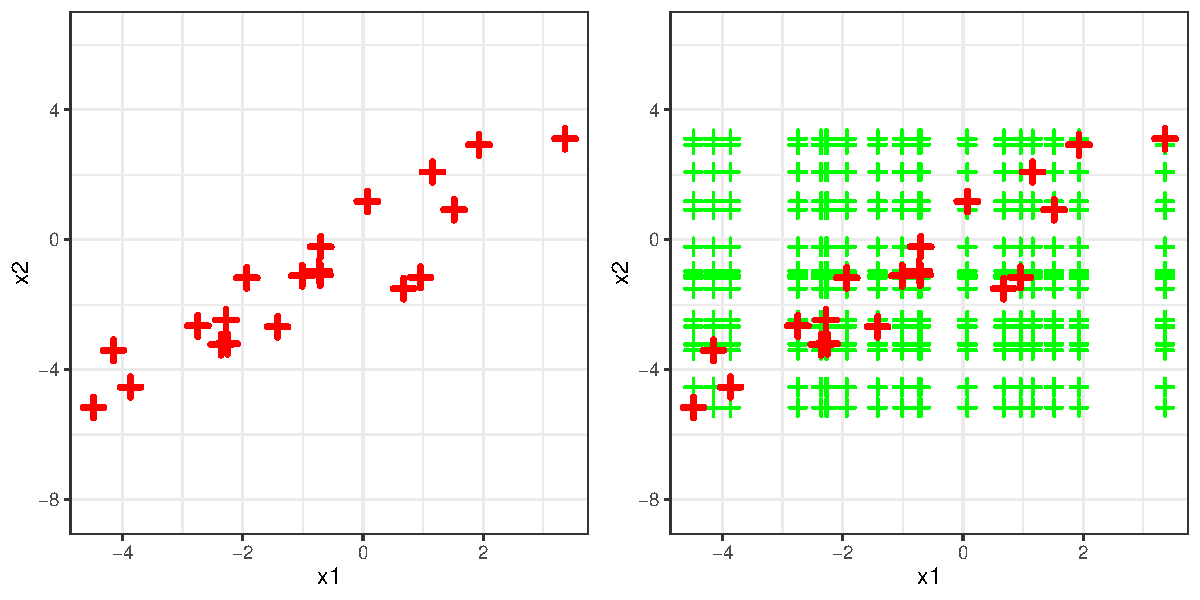
\includegraphics[width=0.8\textwidth]{figure_man/pd_grid}
%\tiny{Source: Figure taken from Apley et al. (2020)}
%\end{center}

%In case of strongly correlated features $x_1$ and $x_2$, PD plots \textbf{average predictions} of artificial data points that are unlikely in reality (red).

\begin{itemize}
    \item PD plots \textbf{average over predictions} of artificial points that are out of distribution/ unlikely (red)\\
    $\Rightarrow$ Can lead to misleading / biased interpretations, especially if model also contains interactions
    \item Not wanted if interest is to interpret effects within data distribution
\end{itemize}
%If features are correlated, PD plots \textbf{average predictions} of artificial points that are unlikely (red).
%\textbf{But:} This might be undesired if interest is to interpret effects within data distribution.
%This can be an undesired property if the model contains interactions and one is interested in interpreting effects w.r.t. the data distribution.

%\lz

%\textbf{Question:} Can we avoid the extrapolation issue by averaging only over points in an appropriate neighborhood? % of a specific point $x_1$? %, i.e., using the conditional distribution at

\end{frame}


\begin{frame}{Motivation - Correlated Features}

%TODO: Example what can go wrong with PDPs and NNs

Example: Fit an NN to $5000$ simulated data points with $x \sim Unif(0,1)$, $\epsilon \sim N(0, 0.2)$ and

\centerline{$y = x_1 + x_2^2 + \epsilon$, where
$x_1 = x + \epsilon_1$, 
$x_2 = x + \epsilon_2$ and $\epsilon_1, \epsilon_2 \sim N(0, 0.05)$.}

\begin{columns}[T, totalwidth=\textwidth]
\begin{column}{0.65\textwidth}
\centering
\only<1>{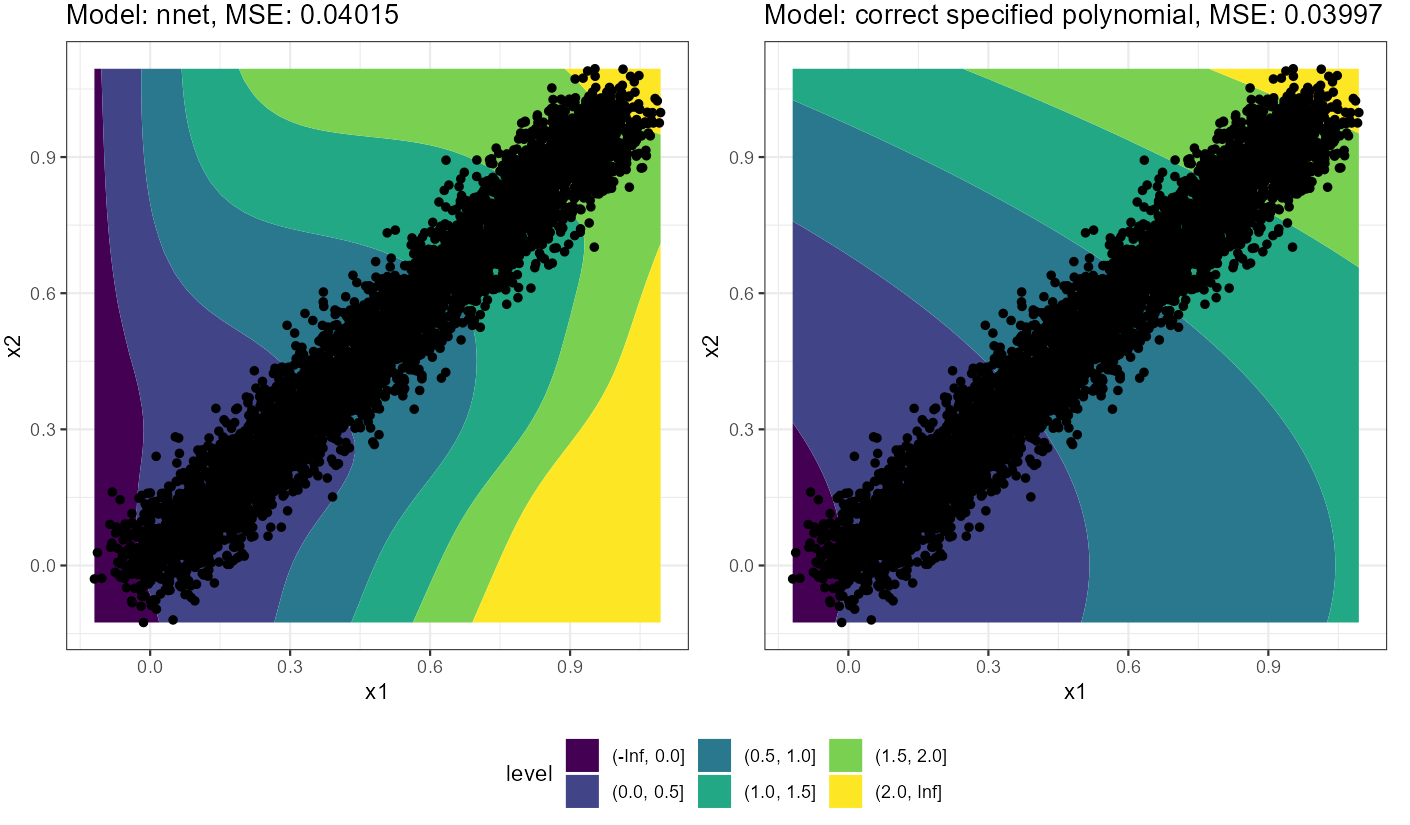
\includegraphics[width=\textwidth]{figure/ale_vs_pdp_surf}}
\only<2>{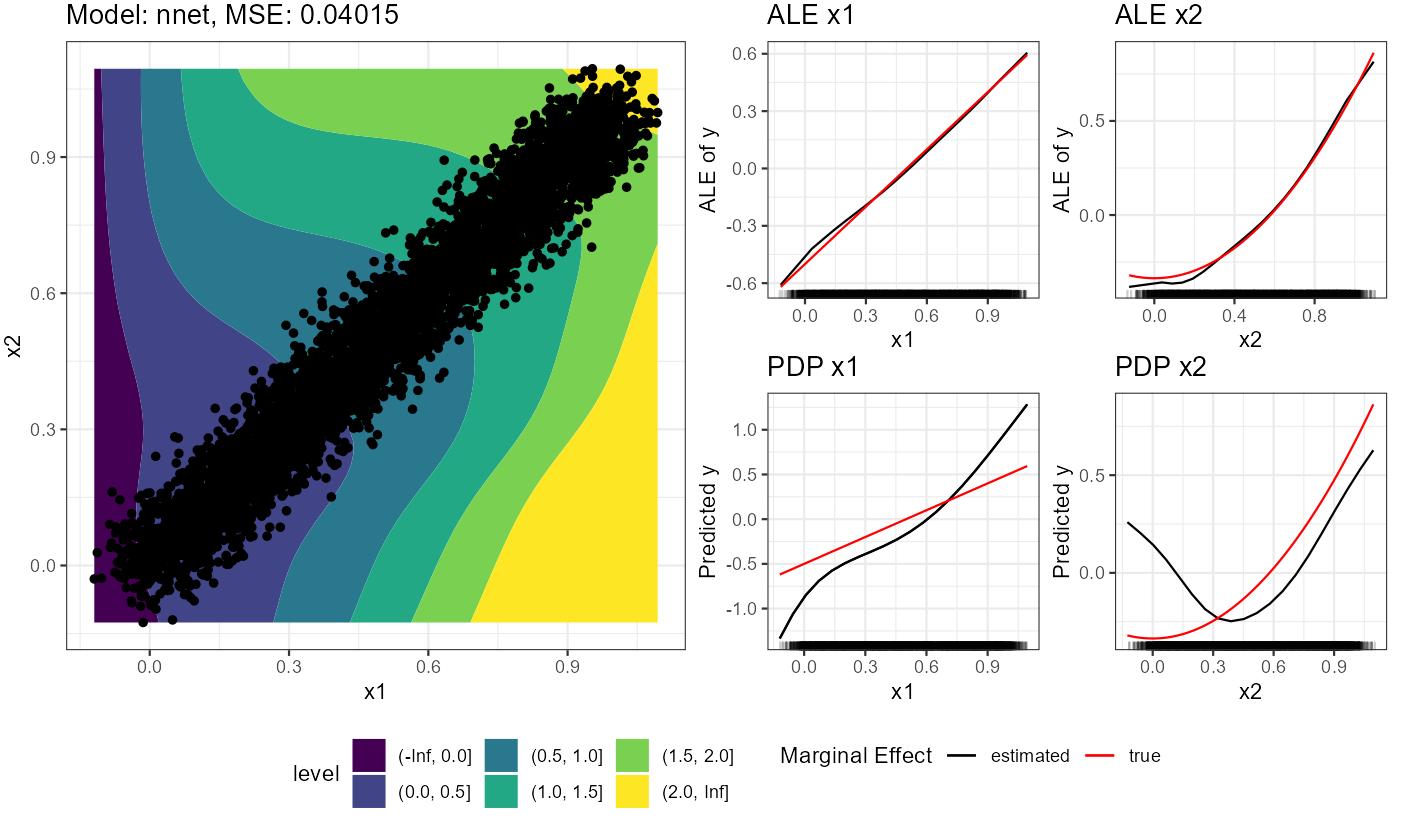
\includegraphics[width=\textwidth]{figure/ale_vs_pdp_nn}}
\end{column}
\begin{column}{0.35\textwidth}
%What went wrong here?

\begin{itemize}
\item Test error (MSE) of NN is comparable to other models
\item NN contains interactions (see complex pred. surface)
%\item ALE shows a linear effect for $x_1$ and quadratic effect for $x_2$\\
%$\Rightarrow$ In line with ground truth %Match true effects of DGP
%\item PDP shows expected model behaviour but does not recover effects of DGP \\
%$\Rightarrow$ Due to averaging of artificial points outside data distribution
\item<2> ALE in line with ground truth
\item<2> PDP does not reflect ground truth effects of DGP well \\
$\Rightarrow$ Due to interactions and averaging of points outside data distribution
\end{itemize}

\end{column}
\end{columns}

\end{frame}

\begin{frame}{M Plot vs. PD plot}

% \begin{center}
% 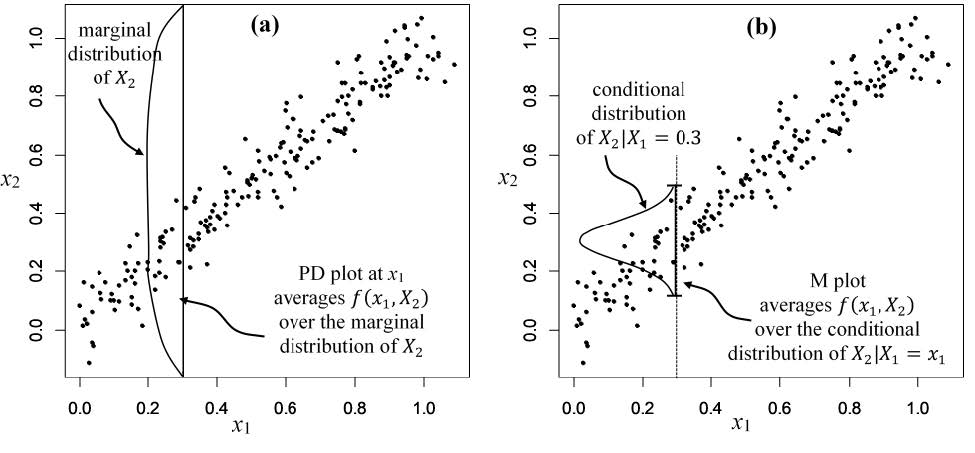
\includegraphics[width=0.7\textwidth]{figure_man/PD_M.jpg}\\
% \tiny{Source: Figure taken from Apley et al. (2020)}
% \end{center}

\begin{columns}[T, totalwidth=\textwidth]
\visible<1-2>{\begin{column}{0.5\textwidth}
\vspace*{-1em}
\centering
\textbf{a) PD plot}
\includegraphics[width=0.9\textwidth]{figure/ale_pdplot}
\end{column}
}
\visible<2>{\begin{column}{0.5\textwidth}
\vspace*{-1em}
\textbf{b) M plot}
\centering
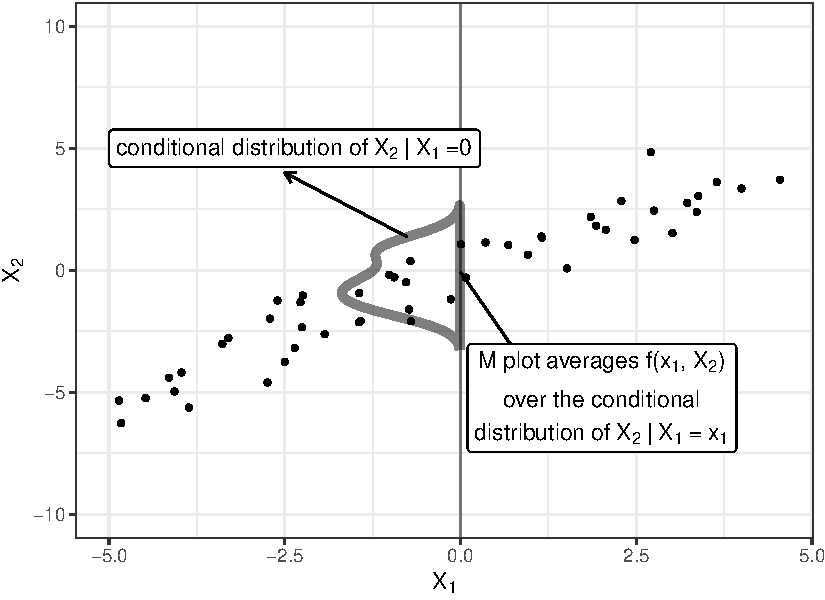
\includegraphics[width=0.9\textwidth]{figure/ale_mplot}
\end{column}
}
\end{columns}

\begin{enumerate}[<+->]
%\item[a)] PD plot $\fh_{1, PD}(x_1) = \hat{\E}_{\xv_2} \left( \fh(x_1, \xv_2) \right) = \frac{1}{n} \sum_{i=1}^n \fh(x_1, \xv_2^{(i)})$
%\item[b)] M plot $\fh_{1, M}(x_1) = \hat{\E}_{\xv_2|\xv_1} \left( \fh(x_1, \xv_2) \middle| \xv_1\right) = \frac{1}{|N(x_1)|} \sum\limits_{i \in N(x_1)} \fh(x_1, \xv_2^{(i)})$, where $N(x_1) = \{i: x_1^{(i)} \in [x_1 - \epsilon, x_1 + \epsilon]\}$ is an index set referring to observations in an appropriate neighborhood of feature value $x_1$.
\item[a)] PD plot $\E_{\xv_2} \left( \fh(x_1, \xv_2) \right)$ is estimated by $ \fh_{1, PD}(x_1) = \frac{1}{n} \sum\limits_{i=1}^n \fh(x_1, \xv_2^{(i)})$
\item[b)] M plot $\E_{\xv_2|\xv_1} \left( \fh(x_1, \xv_2) \middle| \xv_1\right)$ is
estimated by $\fh_{1, M}(x_1) = \textstyle\frac{1}{|N(x_1)|} \sum_{i \in N(x_1)} \fh(x_1, \xv_2^{(i)}),$
where index set $N(x_1) = \{i: x_1^{(i)} \in [x_1 - \epsilon, x_1 + \epsilon]\}$ refers to observations with feature value close to $x_1$. %in an appropriate neighborhood of feature value $x_1$.
\end{enumerate}
\end{frame}

\begin{frame}{M Plot vs. PD plot}

\begin{columns}[T, totalwidth=\textwidth]
\begin{column}{0.5\textwidth}
\centering
\includegraphics[width=0.9\textwidth]{figure/ale_scatter}
\end{column}
\begin{column}{0.5\textwidth}
\centering
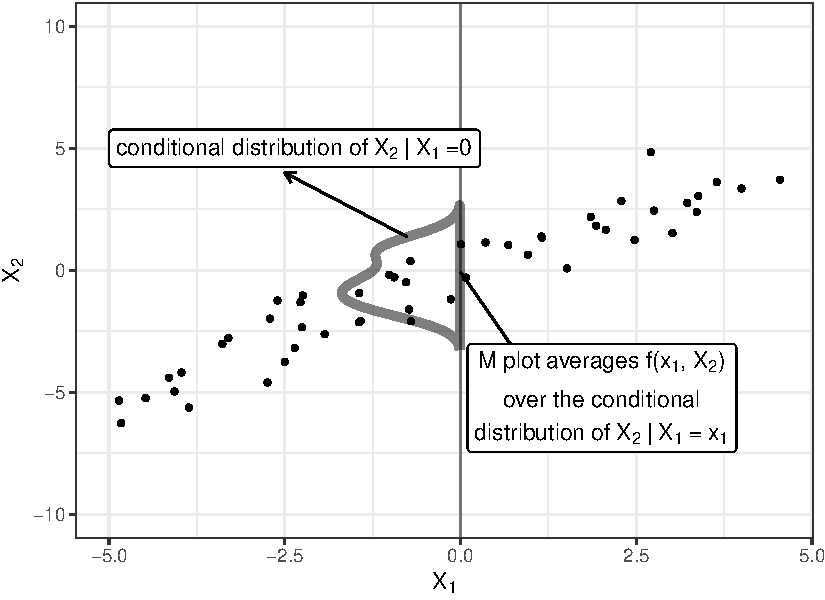
\includegraphics[width=0.9\textwidth]{figure/ale_mplot}
\end{column}
\end{columns}

%\textbf{Answer:} Yes, we could.
%\textbf{Recall:} Marginal plots (M plots) do this by averaging (i.e., marginalizing) over the conditional distribution $\P(\xv_2|x_1)$.
%\textbf{Recall:}

\begin{itemize}
    \item M plots average predictions over conditional distribution (e.g., $\P(\xv_2|x_1)$)\\
    $\Rightarrow$ Averaging predictions close to data distribution avoid extrapolation issues
    \item \textbf{But:} M plots suffer from omitted-variable bias (OVB)
\begin{itemize}
\item Because of the conditioning M plots contain effects of other dependent features
\item Useless in assessing a feature's marginal effect if feature dependencies are present
\end{itemize}
\end{itemize}

% in case of dependent features.

%M plots average over the conditional distribution $x_2|x_1$. However, the M plot of $x_1$ also includes the marginal effect of other dependent features $\Rightarrow$ We don't want this.
% do not include the marginal effect of the considered feature but
% mixture of its marginal effect and the marginal effects of all dependent features
\end{frame}

\begin{frame}{M Plot vs. PD plot - OVB Example}
%\vspace*{-\topsep}
%\vspace*{-3\lineskip}

\begin{center}
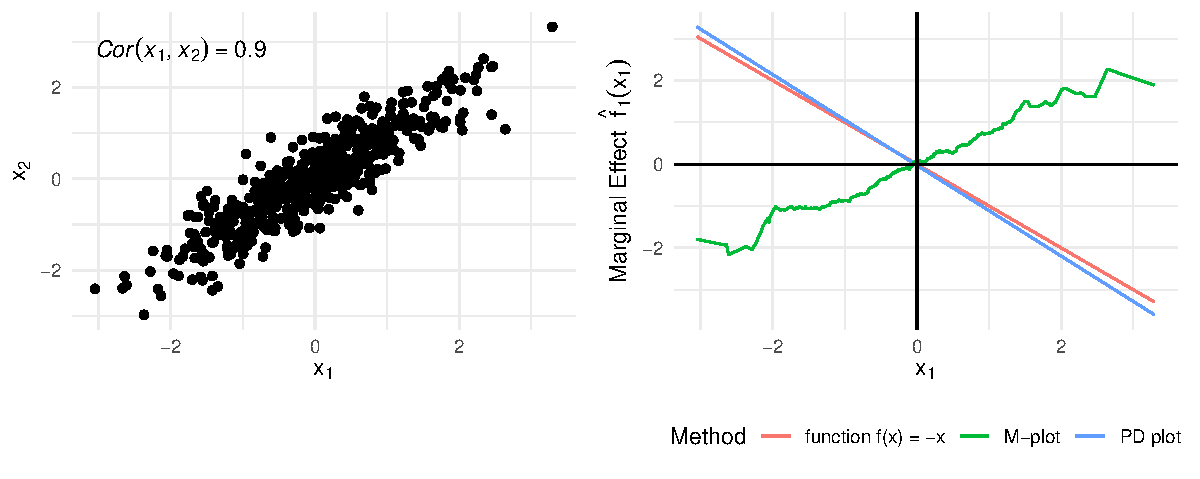
\includegraphics[width=0.9\textwidth]{figure/pd_vs_mplot}
\end{center}

\textbf{Illustration:} Fit LM on 500 i.i.d. observations with features $x_1, x_2 \sim N(0,1)$, $Cor(x_1, x_2) = 0.9$ and $$y = -x_1 + 2 \cdot x_2 + \epsilon, \; \epsilon \sim N(0,1).$$

\textbf{Results:} M plot of $x_1$ also includes marginal effect of all other dependent features (here: $x_2$)
\end{frame}

\begin{frame}{Idea: Integrating Partial Derivatives}

\textbf{Idea:} To remove unwanted effects of other features, take partial derivatives (local effects) of prediction function w.r.t. feature of interest and integrate (accumulate) them w.r.t. the same feature

\begin{itemize}
\item[$\Rightarrow$] Computing the partial derivative of $\fh$ w.r.t. $\xv_j$ removes other main effects
\item[$\Rightarrow$] Integrating again w.r.t. $\xv_j$ recovers the original main effect of $\xv_j$
\end{itemize}

\pause %\lz

\textbf{Example:}
\begin{itemize}[<+->]
\item Consider an additive prediction function: $$\fh(x_1, x_2) = 2x_1 + 2x_2 - 4x_1 x_2$$
\item Partial derivative of $\fh$ w.r.t. $x_1$:
$\frac{\partial \fh(x_1, x_2)}{\partial x_1} = 2 - 4x_2$
\item Integral of partial derivative ($z_0 = \min(x_1)$):
$$\int_{z_0}^{x} \frac{\partial \fh(x_1, x_2)}{\partial x_1} dx_1 = \left[2x_1 - 4x_1 x_2\right]_{z_0}^{x}$$
\item We removed the main effect of $x_2$, which was our goal % (Note: interaction is still there)
\end{itemize}
\end{frame}
    

\endlecture
\end{document}
